\documentclass[11pt, a4paper]{article}

\usepackage{amsmath, amsthm, amssymb}
\usepackage[top=0.8in, bottom=0.8in, left=0.8in, right=0.8in]{geometry}
\usepackage{graphicx}
\usepackage{float}
\usepackage{booktabs}
\usepackage{caption}
\usepackage{xcolor}
\usepackage[colorlinks=true, linkcolor=blue!70!black, urlcolor=blue!70!black, filecolor=red!75!black]{hyperref}
\usepackage{tikz}
\usetikzlibrary{arrows.meta, positioning, shapes.geometric, calc, patterns}

\captionsetup{font=small, labelfont=bf, skip=4pt}

\newtheorem{theorem}{Theorem}
\newtheorem{proposition}{Proposition}
\newtheorem{assumption}{Assumption}
\newtheorem{remark}{Remark}

\title{\vspace{-1.2em}\Large\textbf{Resilient I-Bug Navigation under Intermittent Signal Spoofing}\\
\large\textbf{An Illustrated, Accessible Edition for Demystifying the Mathematics and Terminology}}

\author{
  \textbf{Tsuriel Vizel} \quad \textbf{Avraham Guez} \\
  \small Supervisor: Dr.\ Andrey Zhitnikov $\cdot$ Technion -- Israel Institute of Technology
}
\date{}

\begin{document}

\maketitle

\begin{abstract}
\noindent
\textbf{The Paper in One Sentence:} Imagine a simple blindfolded robot trying to reach a radio beacon inside an unknown obstacle course using only a touch bumper and a "Hot-or-Cold" signal-strength meter. We show how an intermittent "spoofing" transmitter can trick the robot into walking in circles forever—and how the robot can use the physics of its own top speed to catch the fake signal and reach the goal without adding a single new sensor!

\smallskip
\noindent
\textbf{Accessible Scientific Abstract:}
Minimalist autonomous robots operating in GPS-denied environments rely on local sensor feedback rather than global coordinates or \textbf{odometry} (wheel-rotation distance tracking). The \textbf{I-Bug} algorithm achieves guaranteed target convergence using only a binary contact sensor and a \textbf{scalar} signal-intensity sensor (a sensor that reports a single number—strength—without direction). However, in noncoherent sensing settings where the receiver observes the \textbf{additive sum} of multiple emitters, intensity-based navigation is acutely vulnerable to intermittent adversarial \textbf{spoofing}. An additive spoofing transmitter warps the spatial direction of steepest signal increase (\textbf{the gradient}) in free space and injects false signal peaks along obstacle boundaries, trapping standard I-Bug agents in perpetual loops. We present a kinematics-based temporal \textbf{anomaly filter} and two counter-strategies—a \textit{Cautious} strategy that conditionally preserves the exact active path and convergence guarantee of benign I-Bug, and a fast open-loop \textit{Inertial} heuristic—requiring zero additional hardware. We prove mathematically that under intermittent step-spoofing (Assumptions~1--2), the Cautious strategy reproduces the exact active trajectory of a no-attack I-Bug robot, and we prove that freezing memory alone while continuing boundary motion can still fail due to topological phase-locking (\textbf{resonance}). Paired evaluations across $1,000,000$ randomized 2D obstacle environments show that the unmodified Naive I-Bug baseline succeeds in only $54.68\% \pm 0.10\%$ of runs, the Inertial heuristic achieves $99.61\% \pm 0.01\%$ success while cutting mean steps by $20.5\%$, and the Cautious strategy achieves a $\mathbf{100.00\%}$ observed success rate, matching the no-attack I-Bug reference.
\end{abstract}

\section*{Reader's Guide: Quick Mathematical Notation \& Terminology Key}
To make both this edition and the original research paper effortless to read, here is what every mathematical symbol in the equations actually means:
\begin{itemize}
    \item \textbf{Sets and Spaces ($\in, \subset, \mathbb{R}^2$):} $\mathbb{R}^2$ simply means a flat 2D plane with $(x, y)$ coordinates. Writing $\mathcal{W} \subset \mathbb{R}^2$ means our arena $\mathcal{W}$ is a bounded region inside that 2D plane. $\mathcal{O} = \{O_1, \dots, O_M\}$ is the collection of $M$ walls/obstacles, and $\mathcal{F} \subset \mathcal{W}$ (for \textit{Free space}) is the navigable floor where the robot does not collide with any obstacle. Writing $p \in \mathcal{F}$ simply reads: ``position $p$ is inside the collision-free space $\mathcal{F}$.''
    \item \textbf{Euclidean Distance ($\|p - p_t\|_2$):} The double bars with a subscript $2$ denote the straight-line distance (via the Pythagorean theorem, $\sqrt{(x-x_t)^2 + (y-y_t)^2}$) between the robot's position $p$ and the target beacon $p_t$.
    \item \textbf{Scalar vs.\ Vector:} A \textit{scalar} is a single number (e.g., signal strength $S = 0.25$). A \textit{vector} has both magnitude and direction (an arrow). The robot's intensity sensor measures only a scalar—it does not directly tell the robot which direction the beacon is!
    \item \textbf{Gradient ($\nabla_p S$) and Partial Derivatives ($\partial_x S, \partial_y S$):} The upside-down triangle $\nabla_p S$ is the \textit{gradient vector}: an arrow pointing in the direction where signal strength $S$ increases fastest (``steepest uphill''). The symbol $\partial_x S$ asks: ``how much does $S$ change if I take a tiny step along the $x$-axis?'', and $\partial_y S$ asks the same along the $y$-axis.
    \item \textbf{Logical \& Rounding Symbols ($\iff, \lor, \lceil \cdot \rceil$):} $\iff$ means ``if and only if''; $\lor$ means logical ``OR'' (at least one condition holds); and $\lceil x \rceil$ is the \textit{ceiling function}, which rounds $x$ up to the nearest whole integer (e.g., $\lceil 2.1 \rceil = 3$).
\end{itemize}

\hrule
\medskip

\section{Introduction \& Threat Model: Navigating by ``Hot-and-Cold'' and How Spoofing Breaks It}
Classical \textit{Bug} algorithms describe how a minimalist robot—like an insect walking toward a light and feeling its way around obstacles—can reach a goal in an unknown room \cite{lumelsky1987path, kamon1998tangentbug}. The \textbf{I-Bug} (``Intensity-Bug'') algorithm pushes sensor minimalism to the theoretical limit \cite{taylor2009ibug, taylor2014intensity}: a disk-shaped robot of radius $r_c > 0$ has no GPS, no map, and no wheel odometer. It navigates a bounded workspace $\mathcal{W} \subset \mathbb{R}^2$ containing obstacles $\mathcal{O} = \{O_1, \dots, O_M\}$ (with free space $\mathcal{F} \subset \mathcal{W}$) using only a local contact bumper and a scalar sensor measuring signal strength from an unknown target beacon $p_t \in \mathcal{F}$.

In benign (no-attack) conditions, the target signal strength decays inversely with distance:
\begin{equation*}
    m(p - p_t) = \|p - p_t\|_2^{-1} = \frac{1}{\|p - p_t\|_2},
\end{equation*}
and the mission succeeds when the robot enters the target capture radius $\|p - p_t\|_2 < R_{\text{reach}}$. Operating in discrete time steps $k \in \mathbb{N}_0$ (step period $\Delta t$, step size $\Delta s = v_{\max}\Delta t$), the robot uses three basic motion primitives (illustrated in Fig.~\ref{fig:ibug_and_spoof}a):
\begin{enumerate}
    \item $u_{\text{ori}}$ (\textbf{Orient to Gradient — Finding ``Warmer''}): How does a robot with a single scalar sensor find the uphill direction? Within one step, it takes tiny local probe readings slightly left/right ($\partial_x S$) and up/down ($\partial_y S$) and computes the uphill compass angle using the two-argument arctangent function $\operatorname{atan2}$:
    \begin{equation}
        \theta_{\nabla}(p, t) = \operatorname{atan2}\!\bigl(\partial_y S(p, t),\, \partial_x S(p, t)\bigr) \pmod{2\pi}.
        \label{eq:grad_angle}
    \end{equation}
    \item $u_{\text{fwd}}$ (\textbf{Move Forward in Free Space — \texttt{MoveToTower}}): While unobstructed, the robot steps straight ahead along heading $\theta_k$. When its bumper hits an obstacle, it records the signal strength at the hit point into a memory threshold variable $i_H \leftarrow \max(S(p_k, t_k), i_H)$, turns right by $90^\circ$ ($\pi/2$ radians), and switches to \texttt{FollowObstacle}.
    \item $u_{\text{fol}}$ (\textbf{Follow Obstacle Boundary — \texttt{FollowObstacle}}): The robot traces the wall perimeter (keeping the wall on its left) while tracking the highest intensity seen along the boundary, $i_{\text{max}}$. Once it has climbed strictly above the hit threshold ($i_{\text{max}} > i_H + \epsilon$, meaning it is closer to the target than where it hit the wall) and then observes the signal starting to drop ($S(p_k, t_k) < i_{\text{max}} - \epsilon$), it knows it has just passed the closest point to the beacon on that obstacle! It updates $i_H \leftarrow i_{\text{max}}$, re-orients via $u_{\text{ori}}$, and leaves the wall back into \texttt{MoveToTower}.
\end{enumerate}

\begin{figure}[H]
\centering
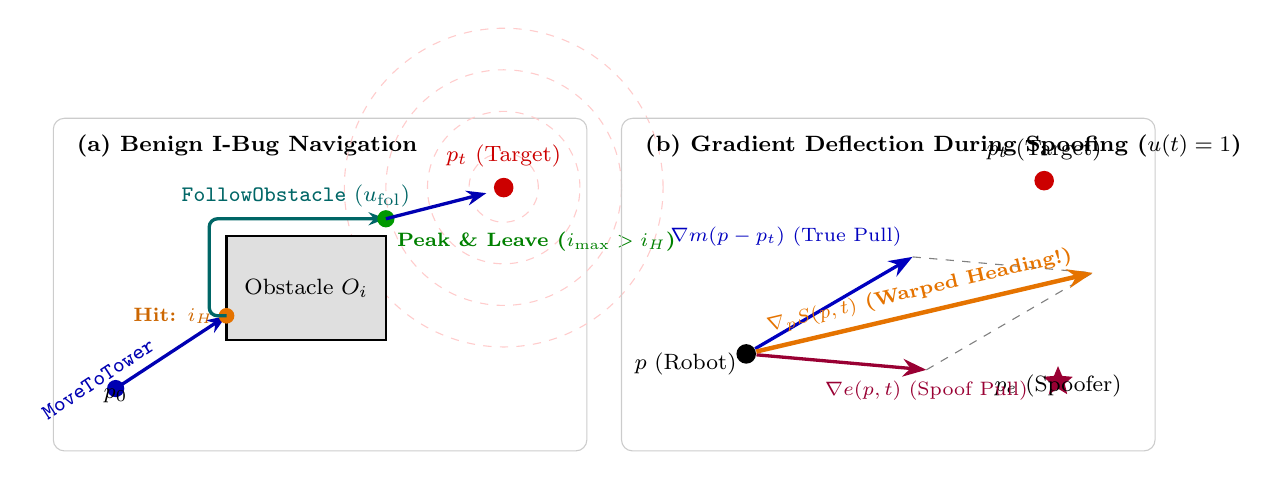
\begin{tikzpicture}[scale=0.88, every node/.style={font=\footnotesize}]
    % --- Panel A: How I-Bug Works ---
    \draw[rounded corners=4pt, gray!40] (-0.3,-0.4) rectangle (7.4,4.4);
    \node[anchor=north west, font=\footnotesize\bfseries] at (-0.1,4.3) {(a) Benign I-Bug Navigation};

    % Target concentric rings
    \foreach \r in {0.5, 1.1, 1.7, 2.3} {
        \draw[red!20, dashed] (6.2,3.4) circle (\r);
    }
    \node[circle, fill=red!80!black, inner sep=2.5pt, label={[red!80!black, above]:$p_t$ (Target)}] (targetA) at (6.2,3.4) {};

    % Obstacle
    \filldraw[fill=gray!25, draw=black, thick] (2.2,1.2) rectangle (4.5,2.7);
    \node at (3.35, 1.95) {Obstacle $O_i$};

    % Robot start
    \node[circle, fill=blue!70!black, inner sep=2.2pt, label={[below]:$p_0$}] (startA) at (0.6,0.5) {};

    % Path to hit point
    \draw[-{Stealth[length=2.5mm]}, blue!70!black, very thick] (0.6,0.5) -- (2.2,1.55) node[midway, above left, sloped] {\texttt{MoveToTower}};
    \node[circle, fill=orange!90!black, inner sep=2pt] at (2.2,1.55) {};
    \node[anchor=east, orange!80!black, font=\scriptsize\bfseries] at (2.15,1.55) {Hit: $i_H$};

    % Follow boundary path
    \draw[-{Stealth[length=2.2mm]}, teal!80!black, very thick, rounded corners=3pt]
        (2.2,1.55) -- (1.95,1.55) -- (1.95,2.95) -- (4.5,2.95);
    \node[teal!80!black, above] at (3.2,2.98) {\texttt{FollowObstacle} ($u_{\text{fol}}$)};

    % Leave point (peak)
    \node[circle, fill=green!60!black, inner sep=2.2pt] at (4.5,2.95) {};
    \node[anchor=north west, green!50!black, font=\scriptsize\bfseries] at (4.52,2.9) {Peak \& Leave ($i_{\max} > i_H$)};

    % Path from leave point to target
    \draw[-{Stealth[length=2.5mm]}, blue!70!black, very thick] (4.5,2.95) -- (5.95,3.32);

    % --- Panel B: Vector Superposition & Gradient Deflection ---
    \begin{scope}[xshift=8.2cm]
        \draw[rounded corners=4pt, gray!40] (-0.3,-0.4) rectangle (7.4,4.4);
        \node[anchor=north west, font=\footnotesize\bfseries] at (-0.1,4.3) {(b) Gradient Deflection During Spoofing ($u(t)=1$)};

        \node[circle, fill=black, inner sep=2.5pt, label={[below left]:$p$ (Robot)}] (rob) at (1.5,1.0) {};
        \node[circle, fill=red!80!black, inner sep=2.5pt, label={[above]:$p_t$ (Target)}] (pt) at (5.8,3.5) {};
        \node[star, star points=5, star point ratio=2.2, fill=purple!80!black, inner sep=1.8pt, label={[below]:$p_e$ (Spoofer)}] (pe) at (6.0,0.6) {};

        \draw[-{Stealth[length=3mm]}, blue!75!black, very thick] (rob) -- (3.9,2.4)
            node[above left, sloped, font=\scriptsize] {$\nabla m(p-p_t)$ (True Pull)};
        \draw[-{Stealth[length=3mm]}, purple!80!black, very thick] (rob) -- (4.1,0.77)
            node[below, sloped, font=\scriptsize] {$\nabla e(p,t)$ (Spoof Pull)};

        \draw[dashed, gray] (3.9,2.4) -- (6.5,2.17);
        \draw[dashed, gray] (4.1,0.77) -- (6.5,2.17);

        \draw[-{Stealth[length=3.2mm]}, orange!90!black, line width=1.6pt] (rob) -- (6.5,2.17)
            node[midway, above, sloped, font=\scriptsize\bfseries] {$\nabla_p S(p,t)$ (Warped Heading!)};
    \end{scope}
\end{tikzpicture}
\caption{\textbf{(a)} How benign I-Bug works: the robot walks uphill toward the beacon (\texttt{MoveToTower}), records intensity $i_H$ upon hitting a wall, follows the perimeter (\texttt{FollowObstacle}) until it detects a peak $i_{\max} > i_H$ at the corner closest to the beacon, and departs toward the goal. \textbf{(b)} When the spoofing transmitter turns on ($u(t)=1$), the sensor observes the sum of both signals, deflecting the steepest-ascent gradient vector $\nabla_p S$ off course.}
\label{fig:ibug_and_spoof}
\end{figure}

\noindent\textbf{The Adversarial Spoofing Model:}
In noncoherent power-sensing systems (radio RSS, optical photodiodes, acoustic energy detectors), multiple transmitters add up at the receiver rather than replacing one another \cite{kerns2014unmanned, psiaki2016gnss}. Suppose a stationary adversarial transmitter at unknown position $p_e \in \mathcal{F}$ broadcasts an intermittent signal of strength $\alpha_e > 0$ controlled by an on/off switch $u(t) \in \{0, 1\}$.

\begin{assumption}[Additive RSS Superposition Field]
\label{assump:superposition}
At position $p \in \mathcal{F}$ and time $t \ge 0$, the sensor measures the sum of the legitimate target intensity $m(p - p_t)$ and the adversarial emission $e(p, t)$:
\begin{equation}
    S(p, t) = m(p - p_t) + e(p, t), \quad e(p, t) = u(t)\,\frac{\alpha_e}{\|p - p_e\|_2}.
    \label{eq:superposition}
\end{equation}
\end{assumption}

When $u(t) = 1$, the attacker corrupts both the scalar reading $S(p, t)$ and its spatial gradient (Fig.~\ref{fig:ibug_and_spoof}b):
\begin{equation}
    \nabla_p S(p, t) = -\frac{p - p_t}{\|p - p_t\|_2^3} - u(t)\,\alpha_e \frac{p - p_e}{\|p - p_e\|_2^3}.
    \label{eq:corrupted_grad}
\end{equation}
This causes two failure mechanisms in standard I-Bug:
\begin{enumerate}
    \item \textbf{Free-Space Gradient Deflection:} During $u_{\text{ori}}$, the robot is pulled along the vector sum of both towers instead of toward $p_t$.
    \item \textbf{Threshold Poisoning ($i_H$):} Even worse, if the robot hits or traces a wall while $u(t) = 1$, it records an artificially inflated threshold $i_H$ (boosted by the attacker's power). Once the attacker switches off ($u(t) \to 0$), the true target signal around that obstacle can never exceed the poisoned $i_H$, trapping the robot on that wall forever!
\end{enumerate}

\section{Physics-Informed Anomaly Detection and Counter-Strategies}

How can a coordinate-free robot detect that the spoofing transmitter just turned on or off? Our defense (inspired by physics-based attack detection \cite{giraldo2018survey, basseville1993detection}) exploits \textbf{timescale separation}: mechanical robot motion is slow ($v_{\max}$), whereas electronic sensor sampling is fast ($\text{kHz}$).

\begin{assumption}[Kinematic Lipschitz Bound vs.\ Temporal Discontinuity]
\label{assump:discontinuity}
Over a high-rate sensor sampling window $\delta t \ll \Delta t$ (maximum physical displacement $\delta s = v_{\max}\delta t \ll R_{\text{reach}}$) while the adversary is off ($u \equiv 0$), the largest possible change in signal intensity from reference $I_{\text{ref}} = 1/d$ caused by the robot's own movement is bounded by:
\begin{equation}
    \Delta I_{\max}(I_{\text{ref}}) = \frac{1}{d - \delta s} - \frac{1}{d} = \frac{\delta s}{d(d - \delta s)} = \frac{\delta s\, I_{\text{ref}}^2}{1 - \delta s\, I_{\text{ref}}}.
    \label{eq:lipschitz}
\end{equation}
Conversely, $u(t)$ switches between $0$ and $1$ such that every active burst lasts at most $T_{\text{on}} \ge 1$ steps and every inactive interval lasts at least $T_{\text{off}} > N_{\text{confirm}}$ steps, producing an instantaneous step jump of at least
\begin{equation}
    e_{\min} := \frac{\alpha_e}{\max_{p \in \mathcal{F}_{\text{nav}}} \|p - p_e\|_2} \ge \frac{\alpha_e}{\operatorname{diam}(\mathcal{W})},
    \label{eq:emin_short}
\end{equation}
which exceeds the kinematic threshold: $e_{\min} > \eta_{\text{spike}} \max_{p \in \mathcal{F}_{\text{nav}}} \Delta I_{\max}(m(p-p_t))$.
\end{assumption}

\begin{remark}[Physical Meaning, Scope, and Safety vs.\ Liveness]
In plain terms, Assumption~\ref{assump:discontinuity} states that if the signal jumps in a millisecond by an amount that would require the robot to teleport a meter forward, an external transmitter must have switched on! Because the detector looks for sharp jumps, it does not cover continuously active or slowly ramped (``adiabatic'') attacks. Furthermore, if an attacker stays on forever ($u(t) \equiv 1$), the Cautious robot will wait indefinitely (denial of service): Theorem~\ref{thm:cautious} guarantees \textbf{safety} (uncorrupted memory and trajectory), while \textbf{liveness} (forward progress) requires the off-intervals $T_{\text{off}} > N_{\text{confirm}}$.
\end{remark}

\begin{figure}[H]
\centering
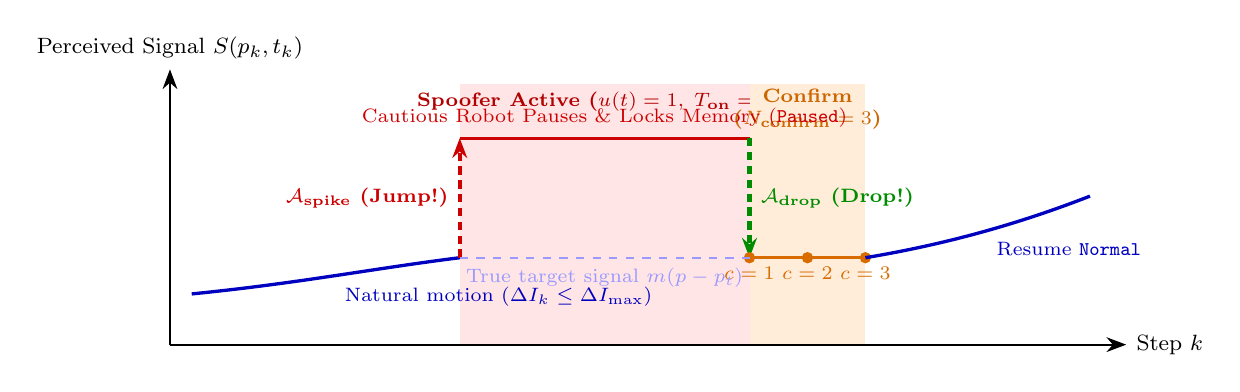
\begin{tikzpicture}[scale=0.92, every node/.style={font=\footnotesize}]
    \fill[red!10] (4.0,0) rectangle (8.0,3.6);
    \node[red!70!black, font=\scriptsize\bfseries] at (6.0, 3.35) {Spoofer Active ($u(t)=1,\; T_{\text{on}}=10$)};

    \fill[orange!15] (8.0,0) rectangle (9.6,3.6);
    \node[orange!80!black, font=\scriptsize\bfseries, align=center] at (8.8, 3.25) {Confirm\\($N_{\text{confirm}}=3$)};

    \draw[-{Stealth[length=2.5mm]}, thick] (0,0) -- (13.2,0) node[right] {Step $k$};
    \draw[-{Stealth[length=2.5mm]}, thick] (0,0) -- (0,3.8) node[above] {Perceived Signal $S(p_k, t_k)$};

    \draw[blue!75!black, very thick] (0.3,0.7) .. controls (1.8,0.85) and (2.8,1.05) .. (4.0,1.2)
        node[midway, below right, font=\scriptsize] {Natural motion ($\Delta I_k \le \Delta I_{\max}$)};

    \draw[-{Stealth[length=2.5mm]}, red!80!black, line width=1.5pt, densely dashed] (4.0,1.2) -- (4.0,2.85)
        node[midway, left, font=\scriptsize\bfseries] {$\mathcal{A}_{\text{spike}}$ (Jump!)};

    \draw[red!80!black, very thick] (4.0,2.85) -- (8.0,2.85)
        node[midway, above, font=\scriptsize] {Cautious Robot Pauses \& Locks Memory (\texttt{Paused})};

    \draw[-{Stealth[length=2.5mm]}, green!55!black, line width=1.5pt, densely dashed] (8.0,2.85) -- (8.0,1.2)
        node[midway, right, font=\scriptsize\bfseries] {$\mathcal{A}_{\text{drop}}$ (Drop!)};

    \draw[orange!85!black, very thick] (8.0,1.2) -- (9.6,1.2);
    \foreach \x/\c in {8.0/1, 8.8/2, 9.6/3} {
        \filldraw[orange!85!black] (\x,1.2) circle (2pt) node[below, font=\scriptsize] {$c=\c$};
    }

    \draw[blue!75!black, very thick] (9.6,1.2) .. controls (10.8,1.4) and (11.8,1.7) .. (12.7,2.05)
        node[midway, below right, font=\scriptsize] {Resume \texttt{Normal}};

    \draw[blue!40, dashed, thick] (4.0,1.2) -- (8.0,1.2) node[midway, below, font=\scriptsize] {True target signal $m(p-p_t)$};
\end{tikzpicture}
\caption{How the anomaly filter and Cautious strategy operate over time: normal motion produces gentle signal changes bounded by $\Delta I_{\max}$. When the attacker switches on, the vertical jump triggers $\mathcal{A}_{\text{spike}}$, freezing the robot and locking its memory until the deactivation drop $\mathcal{A}_{\text{drop}}$ is followed by $N_{\text{confirm}}=3$ clean steps. \textbf{[Watch live simulation animation: \href{run:anomaly_filter_anim.gif}{Click to open \texttt{anomaly\_filter\_anim.gif}} or view \href{run:accessible_paper_online_en.html}{the Online HTML Edition}]}}
\label{fig:anomaly_filter}
\end{figure}

\noindent\textbf{The Anomaly Filter and Three Navigation Strategies (Fig.~\ref{fig:anomaly_filter}):}
At the start of step $k$ (before moving), the filter compares the pre-step reading $I_k^- = S(p_{k-1}, t_k)$ against the previous post-step reading $I_{k-1}^+ = S(p_{k-1}, t_{k-1})$ at the exact same position ($\Delta I_k = I_k^- - I_{k-1}^+$), flagging spikes and drops via:
\begin{align}
    \mathcal{A}_{\text{spike}} &\iff \Delta I_k > \eta_{\text{spike}}\,\Delta I_{\max}(I_{k-1}^+), \qquad (\eta_{\text{spike}} = 2.0), \label{eq:spike} \\
    \mathcal{A}_{\text{drop}} &\iff (-\Delta I_k > 0.15 I_{k-1}^+) \;\lor\; (-\Delta I_k > \eta_{\text{drop}}\Delta I_{\max}(I_k^-)), \qquad (\eta_{\text{drop}} = 1.2). \label{eq:drop}
\end{align}
We compare three strategies:
\begin{enumerate}
    \item \textbf{Naive (Original I-Bug Baseline \cite{taylor2014intensity}):} Has no anomaly filter; trusts $S(p, t)$ blindly at all times.
    \item \textbf{Cautious (``Stop and Lock Memory''):} Upon $\mathcal{A}_{\text{spike}}$, the robot enters \texttt{Paused} mode: it stops moving ($\Delta p_k = 0$) and locks its heading and memory $(i_H, i_{\text{max}}, i_{\text{mem}})$ in a ``vault'' so the spoofed signal cannot corrupt them. Once $\mathcal{A}_{\text{drop}}$ occurs and the signal remains stable for $N_{\text{confirm}} = 3$ steps, it unlocks its state and resumes \texttt{Normal} navigation.
    \item \textbf{Inertial (``Keep Moving Blindly in Open Loop''):} To avoid wasting time standing still, upon $\mathcal{A}_{\text{spike}}$, the robot enters \texttt{InertialMode}: it locks its memory (preventing poisoning), but keeps moving using its last clean heading $\theta_{\text{frozen}}$ in free space (or continues physical wall-following via its contact bumper while suspending the leave-obstacle check) until $\mathcal{A}_{\text{drop}}$ restores \texttt{Normal} mode.
\end{enumerate}

\section{Mathematical Proof \& The Resonance Trap}

\begin{theorem}[Conditional Active-State Trajectory and Convergence Preservation]
\label{thm:cautious}
Under Assumptions~\ref{assump:superposition} and~\ref{assump:discontinuity} with $\eta_{\text{drop}} \le \eta_{\text{spike}}$ and $T_{\text{off}} > N_{\text{confirm}}$, for any workspace $\mathcal{W}$:
\begin{enumerate}
    \item[(i)] After removing the paused steps, the sequence of positions and internal states of the Cautious robot ($\gamma_{\text{cautious}}$) is identical step-by-step to the benign baseline I-Bug trajectory ($\gamma_{\text{ideal}}$) in a world with no attacker ($e \equiv 0$).
    \item[(ii)] Whenever the benign execution reaches $\|p_k - p_t\|_2 < R_{\text{reach}}$ in $N_{\text{ideal}} < \infty$ steps, the Cautious robot is guaranteed to reach the target in at most
    \begin{equation}
        N_{\text{cautious}} \le N_{\text{ideal}} + \left\lceil \frac{N_{\text{ideal}}}{T_{\text{off}} - N_{\text{confirm}}} \right\rceil (T_{\text{on}} + N_{\text{confirm}})
        \label{eq:bound}
    \end{equation}
    total steps.
\end{enumerate}
\end{theorem}

\begin{proof}[Intuitive Proof Breakdown]
\textbf{Step 1 (Exact Switching):} Every time the attacker turns on, the jump exceeds $e_{\min}$ and triggers $\mathcal{A}_{\text{spike}}$ before the robot moves or updates memory. Every time the attacker turns off, the drop triggers $\mathcal{A}_{\text{drop}}$, and after $N_{\text{confirm}} = 3$ stationary checks the robot resumes from the exact state where it paused.
\textbf{Step 2 (Path Identity by Induction):} Because the Cautious robot only takes active steps when $u(t) = 0$, it only ever senses the true target field $m(p - p_t)$. Thus, its 1st active step matches the 1st step of a no-attack robot, its 2nd matches the 2nd, and so on by induction!
\textbf{Step 3 (Step Bound):} Each cycle gives at least $T_{\text{off}} - N_{\text{confirm}} \ge 1$ active walking steps at the cost of at most $T_{\text{on}} + N_{\text{confirm}}$ paused steps, yielding Eq.~\eqref{eq:bound}.
\end{proof}

\begin{proposition}[The Topological Resonance Trap in the Inertial Strategy]
\label{prop:resonance}
Freezing memory alone while continuing boundary motion does not guarantee universal convergence. Suppose the robot orbits an obstacle $O_i$ whose perimeter takes $T_{\text{orbit}}$ steps to circle, and let $\mathcal{A}_L \subset \partial O_i$ be the departure arc where the signal peaks closest to the target. If the orbital period synchronizes with the attacker's cycle period $T_{\text{cycle}}$ such that
\begin{equation*}
    T_{\text{orbit}} = m \cdot T_{\text{cycle}} \quad (\text{for some integer } m \ge 1),
\end{equation*}
and the attacker's active window ($T_{\text{on}}$ steps) covers $\mathcal{A}_L$, the Inertial robot will pass over the exit arc $\mathcal{A}_L$ while ``blind'' (peak detection suspended) on every single lap, trapping it in an infinite loop! (See Fig.~\ref{fig:resonance_diagram}).
\end{proposition}

\begin{figure}[H]
\centering
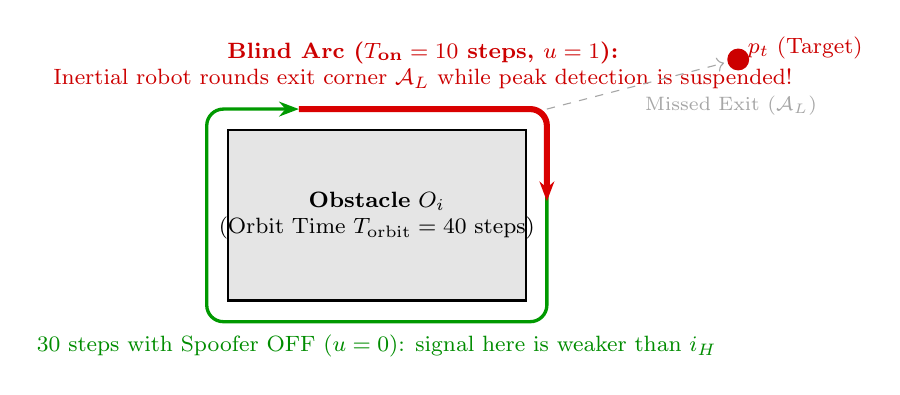
\begin{tikzpicture}[scale=0.9, every node/.style={font=\footnotesize}]
    \filldraw[fill=gray!20, draw=black, thick] (0,0) rectangle (4.2,2.4);
    \node[align=center] at (2.1,1.2) {\textbf{Obstacle} $O_i$\\(Orbit Time $T_{\text{orbit}} = 40$ steps)};

    \draw[-{Stealth[length=2.5mm]}, green!60!black, very thick, rounded corners=6pt]
        (3.2,2.7) -- (4.5,2.7) -- (4.5,-0.3) -- (-0.3,-0.3) -- (-0.3,2.7) -- (1.0,2.7);
    \node[green!55!black, below] at (2.1,-0.35) {$30$ steps with Spoofer OFF ($u=0$): signal here is weaker than $i_H$};

    \draw[-{Stealth[length=2.5mm]}, red!85!black, line width=2.2pt, rounded corners=6pt]
        (1.0,2.7) -- (4.5,2.7) -- (4.5,1.4);
    \node[red!80!black, above, align=center] at (2.75,2.85) {\textbf{Blind Arc ($T_{\text{on}}=10$ steps, $u=1$):}\\Inertial robot rounds exit corner $\mathcal{A}_L$ while peak detection is suspended!};

    \node[circle, fill=red!80!black, inner sep=2.8pt, label={[red!80!black, right]:$p_t$ (Target)}] (pt) at (7.2,3.4) {};
    \draw[dashed, gray!70, ->] (4.5,2.7) -- (7.0,3.35) node[midway, below right, font=\scriptsize] {Missed Exit ($\mathcal{A}_L$)};
\end{tikzpicture}
\caption{Visualizing Proposition~\ref{prop:resonance} (Topological Resonance): circling the obstacle takes $40$ steps—matching the attacker's $40$-step period. Every lap, the $10$-step spoofing burst (red arc) turns on right as the Inertial robot reaches the top-right exit corner $\mathcal{A}_L$, blinding it to the departure peak on every revolution.}
\label{fig:resonance_diagram}
\end{figure}

\section{Large-Scale Evaluation Across $1,000,000$ Mazes}
We built a continuous 2D kinematic simulator in Julia ($\mathcal{W} = [0, 20]^2$, $p_0 = (2, 1)$, $p_t = (18, 18)$, $R_{\text{reach}} = 0.5$, $r_c = \Delta s = 0.3$, $T_{\text{cycle}} = 40$, $T_{\text{on}} = 10$, $T_{\text{off}} = 30$, $\alpha_e = 1.0$, horizon $N_{\max} = 2,000$). Across $1,000,000$ randomized mazes (10--16 overlapping rectangular walls), we ran paired trials of all three strategies alongside a no-attack ($u \equiv 0$) benign reference on the exact same mazes. Under $u \equiv 0$, all three strategies (\textit{Naive}, \textit{Cautious}, and \textit{Inertial}) produced identical step counts in $100\%$ of runs ($100.00\%$ success, mean $132.6$ steps), confirming zero false-positive anomaly detections.

\begin{table}[H]
\centering
\small
\caption{Performance Comparison Across $1,000,000$ Paired Environments}
\label{tab:results}
\resizebox{\linewidth}{!}{%
\begin{tabular}{@{}lcccc@{}}
\toprule
\textbf{Strategy} & \textbf{Success Rate ($95\%$ CI)} & \textbf{Mean Steps (Succ.)} & \textbf{Median [IQR] (Succ.)} & \textbf{Capped Mean ($\bar{N}_{\text{capped}}$)} \\ \midrule
\textit{Benign I-Bug (no attack, all 3 equal)} & \textit{$100.00\%$} & \textit{$132.6$} & \textit{$126.0$ $[108,\, 150]$} & \textit{$132.6$} \\ \midrule
Naive (Unprotected Baseline) & $54.68\% \pm 0.10\%$  & $199.3$ & $153.0$ $[121,\, 205]$ & $1015.4$ \\
Cautious (Stop \& Lock Memory) & $\mathbf{100.00\%}$ ($[99.9996, 100]$) & $193.0$ & $178.0$ $[160,\, 215]$ & $193.0$ \\
Inertial (Open-Loop Continuation) & $99.61\% \pm 0.01\%$  & $\mathbf{153.4}$ & $\mathbf{135.0}$ $[115,\, 168]$ & $\mathbf{160.6}$ \\ \bottomrule
\end{tabular}%
}
\end{table}

\noindent\textbf{How to Read the Statistical Metrics in Table~\ref{tab:results}:}
\begin{itemize}
    \item \textbf{Median [IQR]:} The \textit{median} is the 50th-percentile step count (unaffected by extreme outliers), and the \textit{Interquartile Range (IQR)} in brackets spans the middle $50\%$ of runs (25th to 75th percentile).
    \item \textbf{Capped Mean ($\bar{N}_{\text{capped}}$):} Computing the mean only over successful runs ignores failed runs! Thus $\bar{N}_{\text{capped}}$ averages across all $1,000,000$ runs by assigning failed runs the timeout penalty $N_{\max} = 2,000$.
\end{itemize}

\begin{figure}[H]
    \centering
    \begin{minipage}[t]{0.48\linewidth}
        \centering
        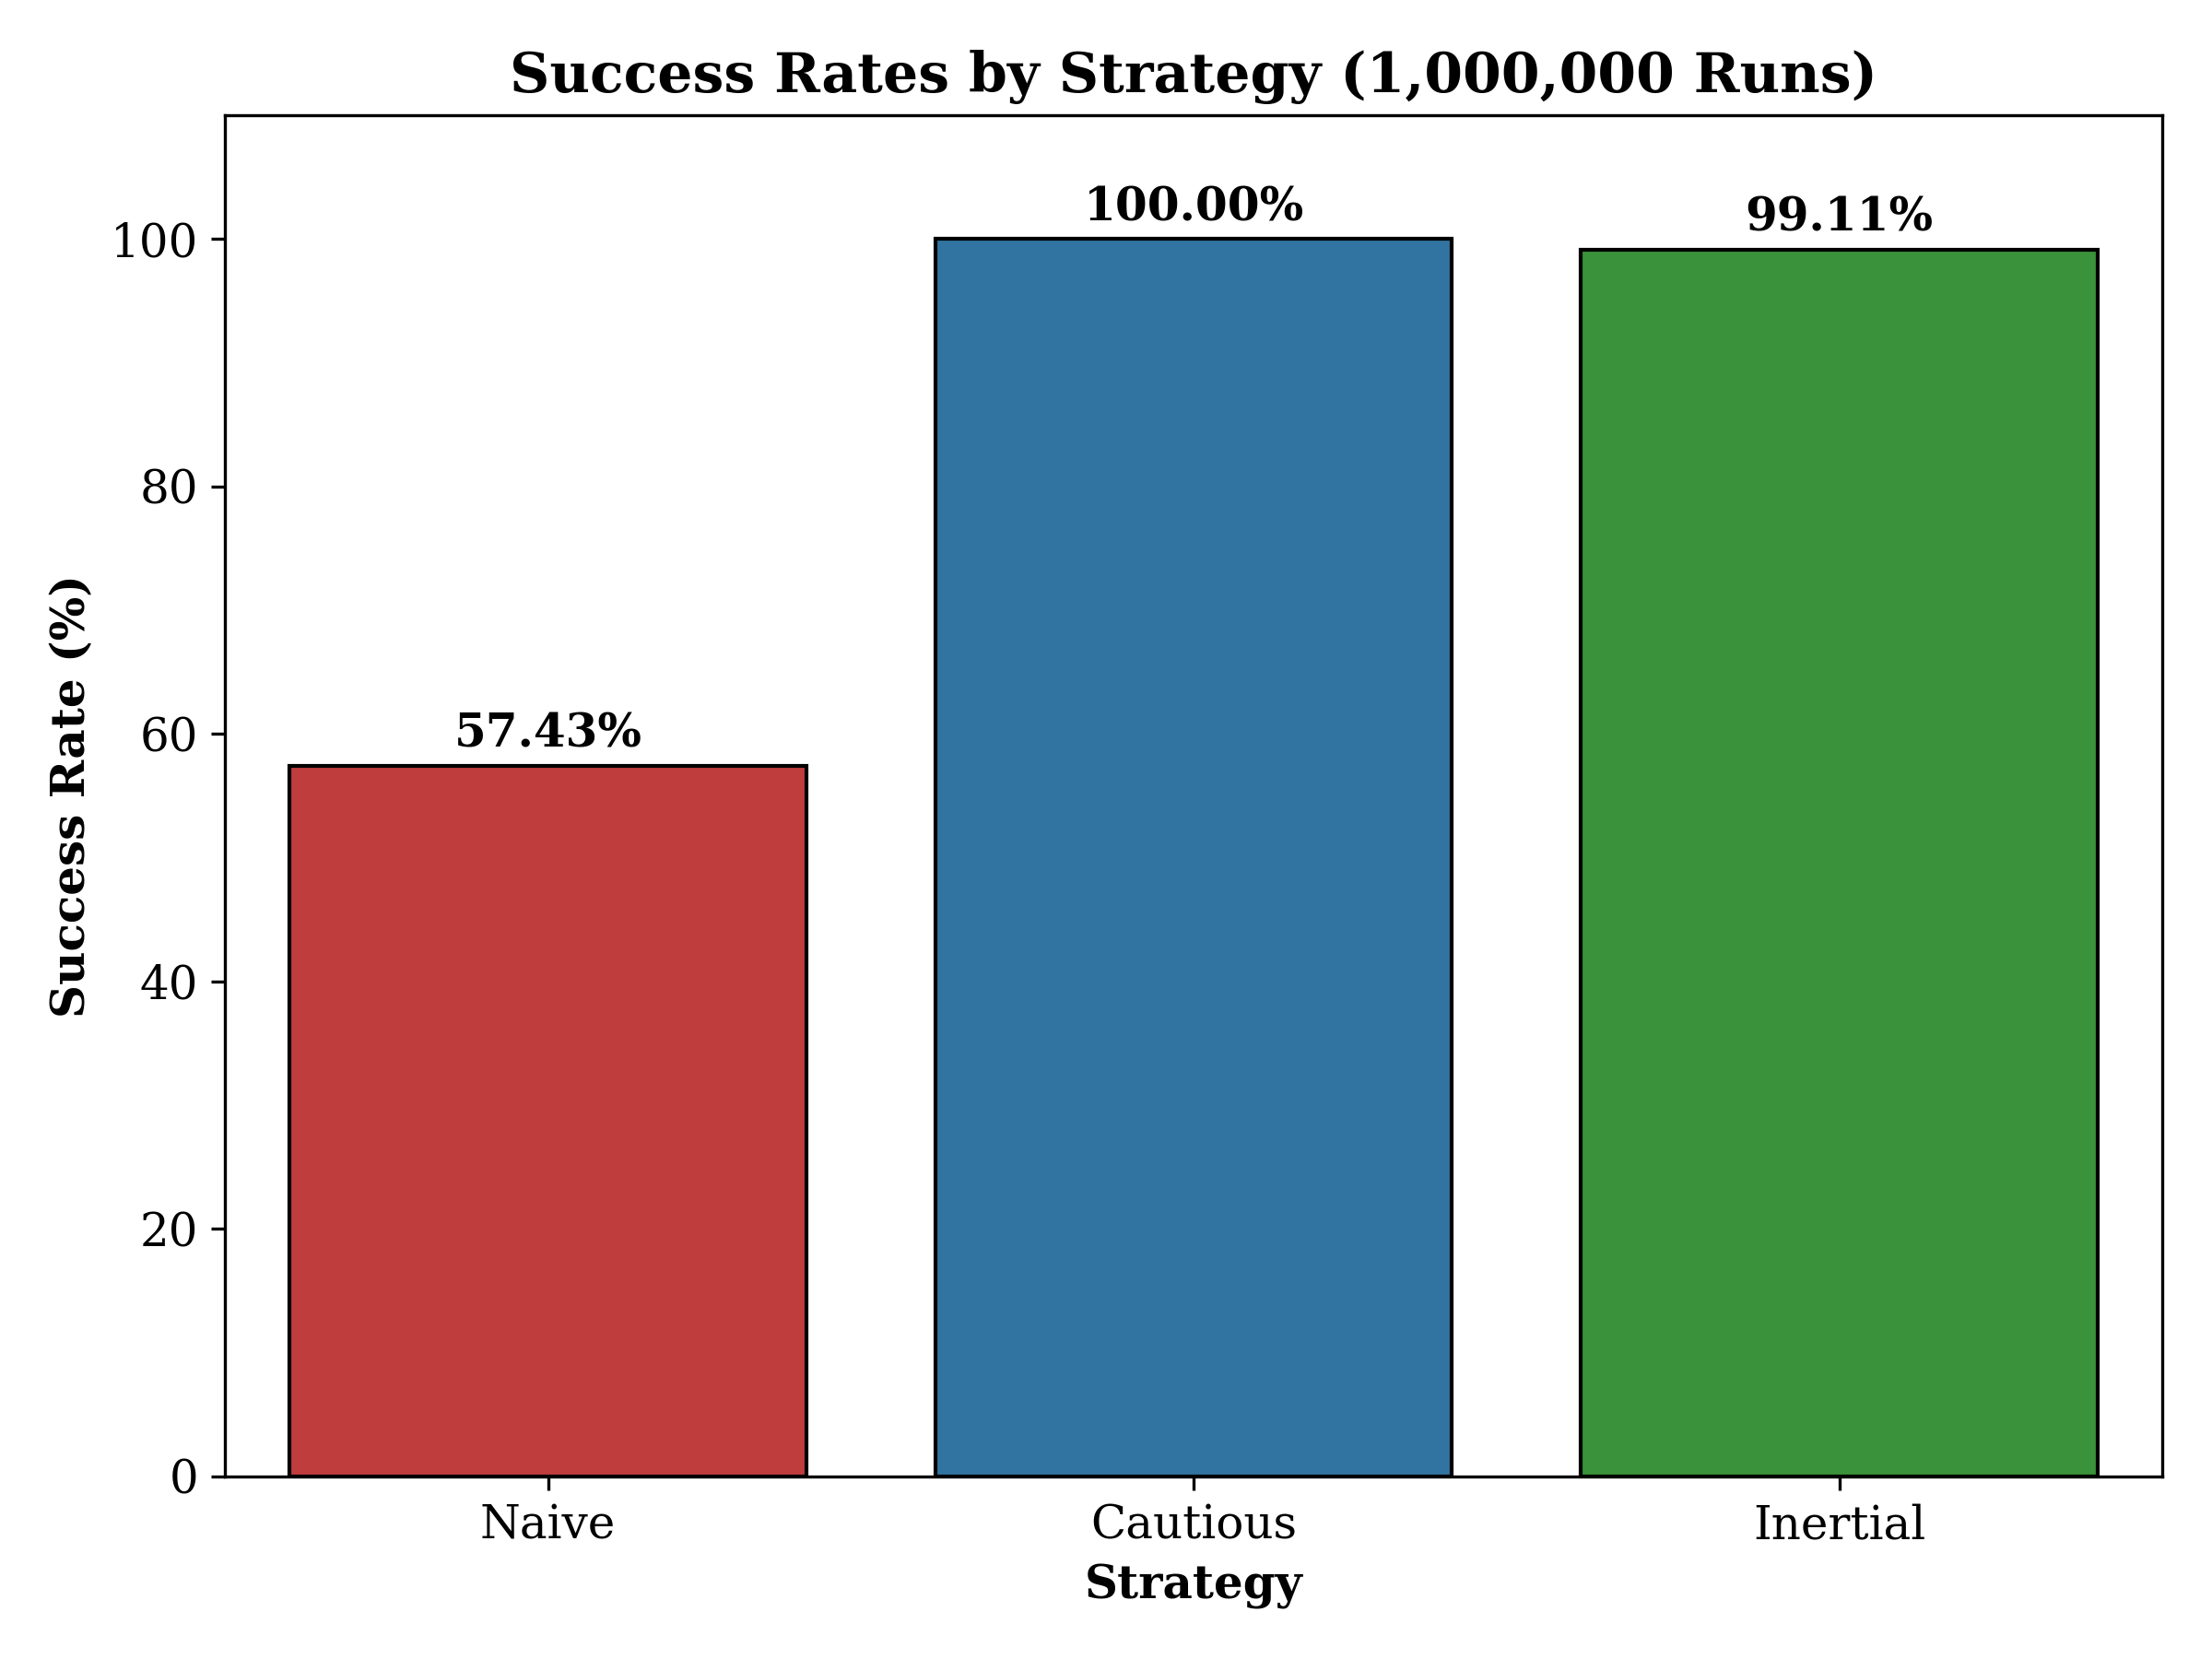
\includegraphics[width=\linewidth]{success_rates.png}
        \caption{Success rates across $1,000,000$ mazes.}
        \label{fig:succ}
    \end{minipage}\hfill
    \begin{minipage}[t]{0.48\linewidth}
        \centering
        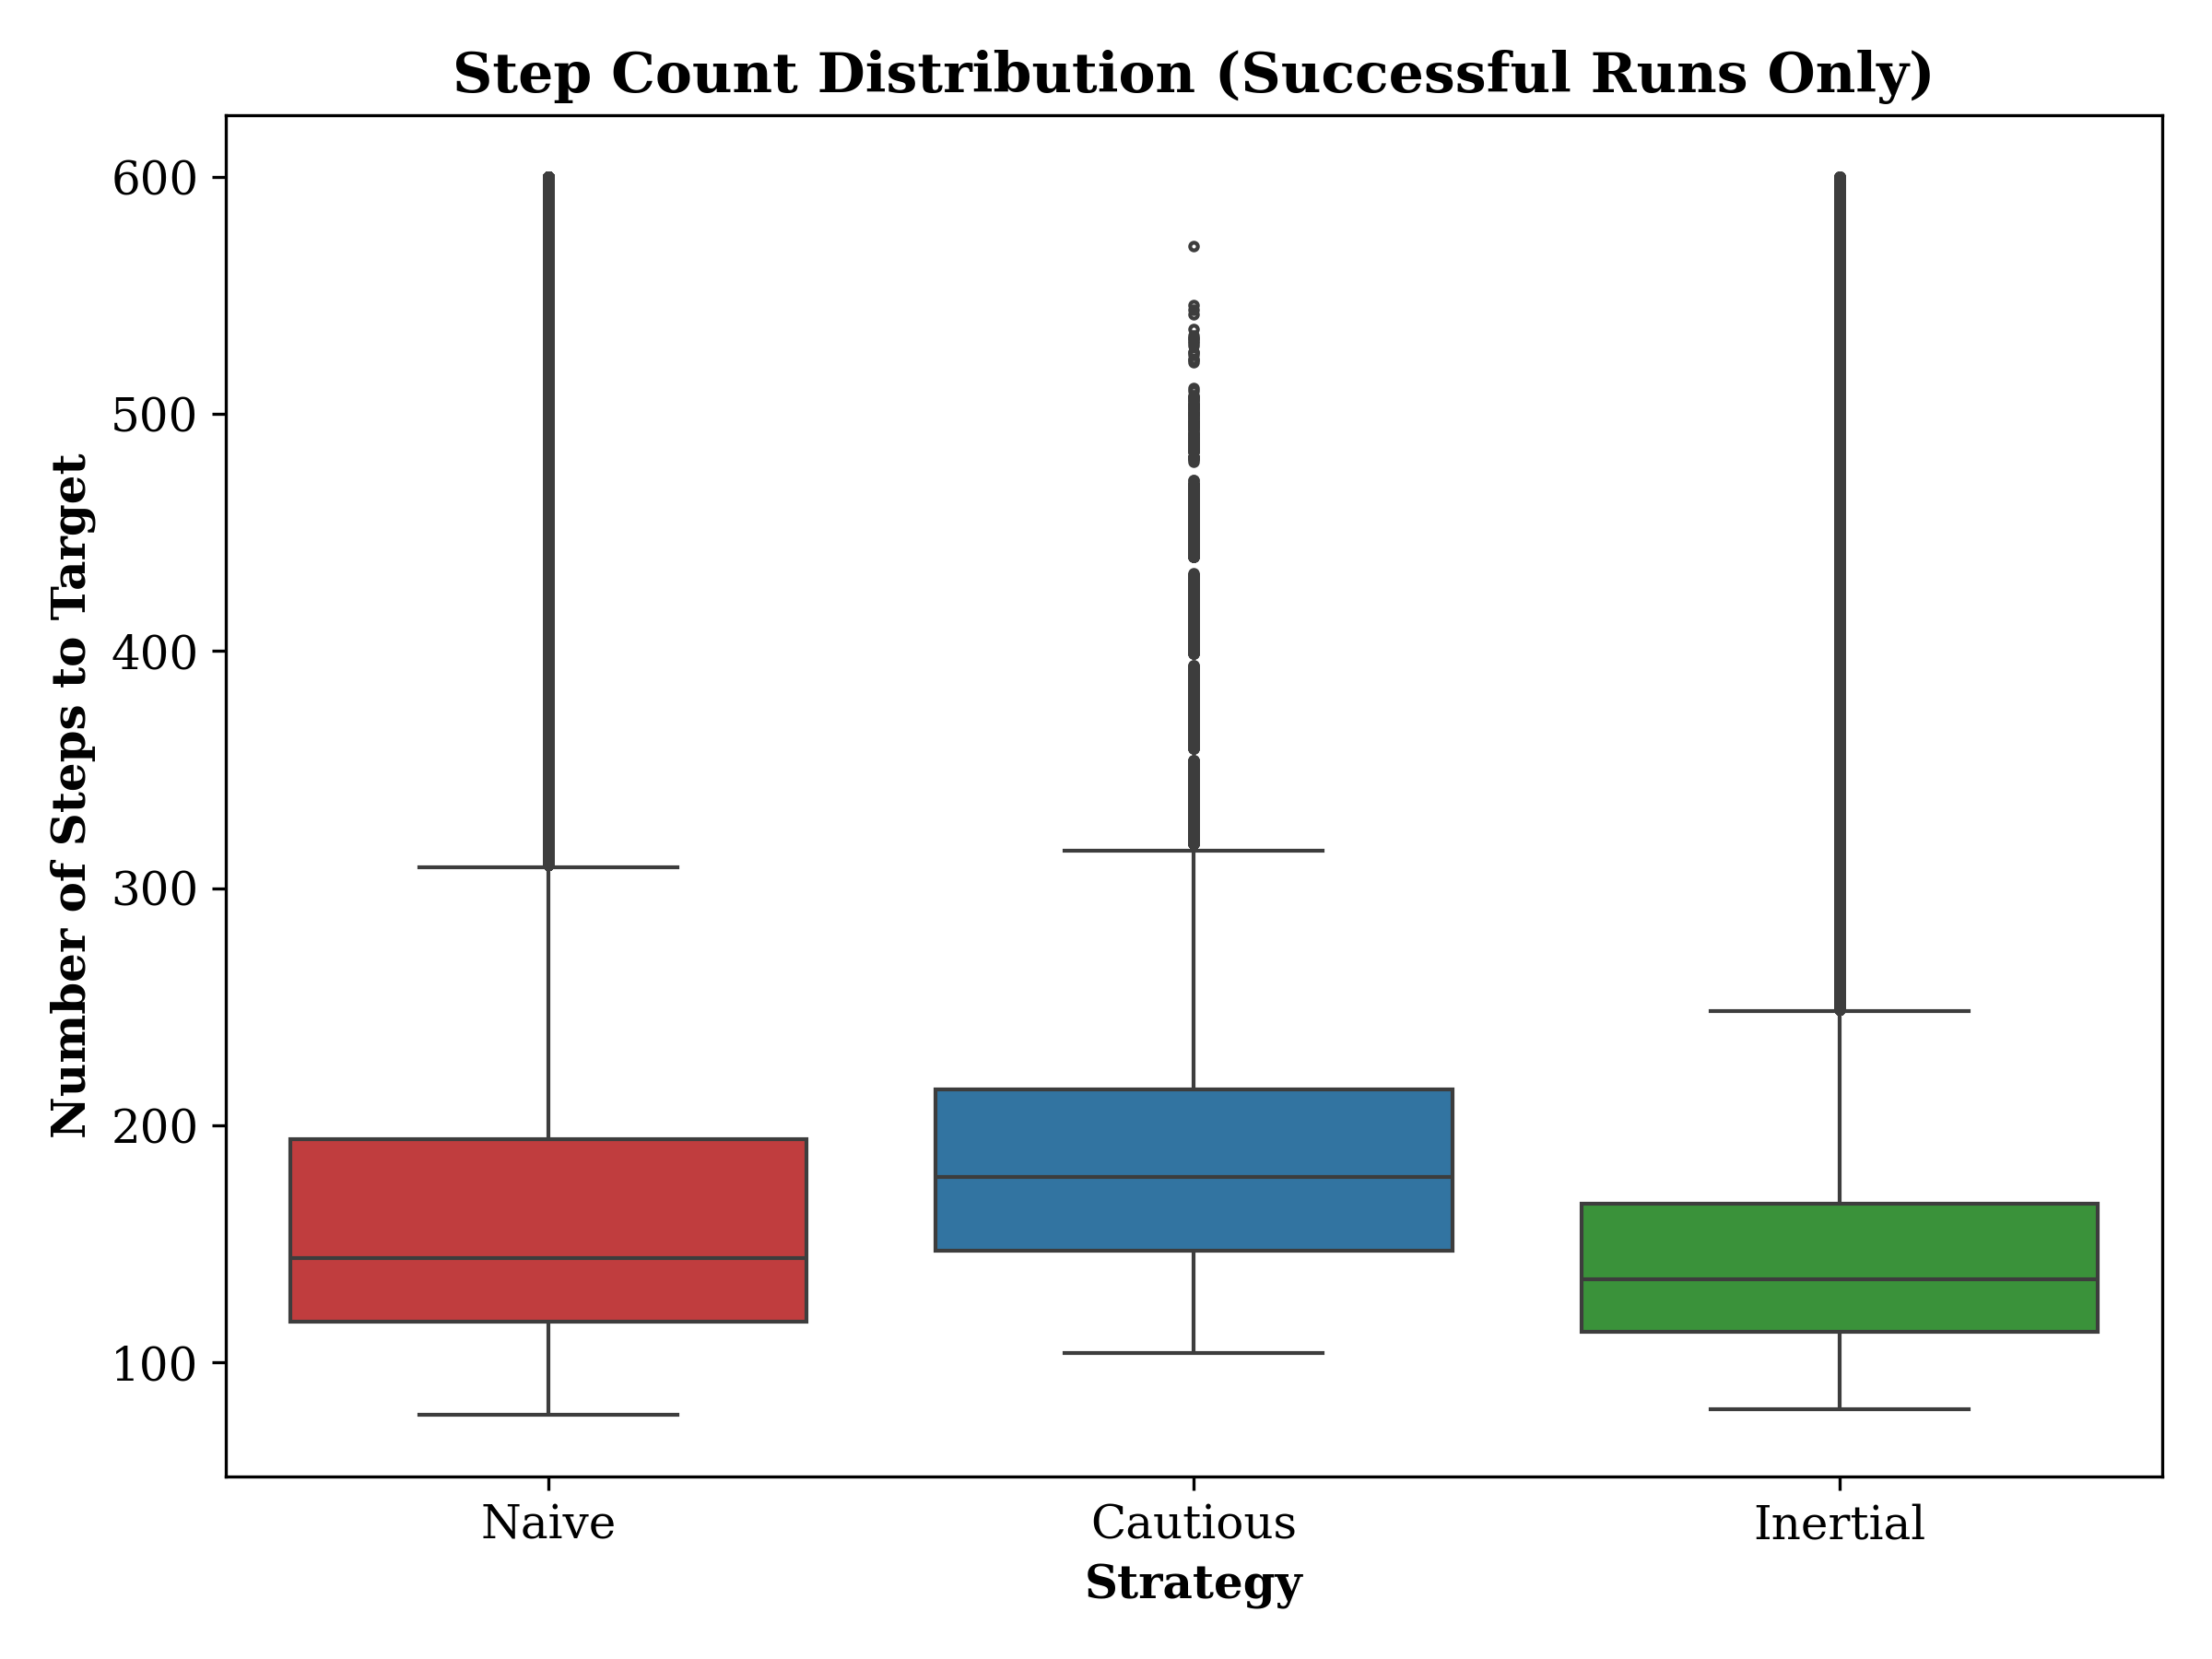
\includegraphics[width=\linewidth]{steps_distribution.png}
        \caption{Step count distribution (successful runs).}
        \label{fig:steps}
    \end{minipage}
\end{figure}

\begin{figure}[H]
    \centering
    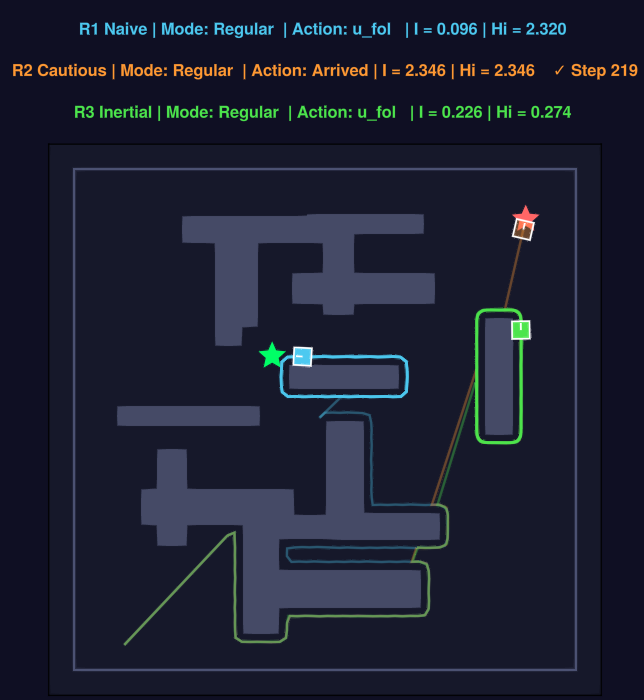
\includegraphics[width=0.68\linewidth]{simulation_trap.png}
    \caption{A real double-failure run from our simulation (RunID 457): \textbf{Naive (cyan)} is threshold-poisoned ($i_H = 1.230$) on the central L-obstacle; \textbf{Inertial (green)} is caught in a 40-step resonant loop on the upper-right rectangle; \textbf{Cautious (orange)} pauses during bursts and reaches the target (red star) in $137$ steps. \textbf{[Watch the step-by-step animated replay: \href{run:simulation_trap_anim.gif}{Click to open \texttt{simulation\_trap\_anim.gif}} or open \href{run:accessible_paper_online_en.html}{the Online HTML Edition}]}}
    \label{fig:trap}
\end{figure}

\begin{thebibliography}{8}
\footnotesize
\setlength{\itemsep}{0pt}
\bibitem{lumelsky1987path}
V.~J. Lumelsky and A.~A. Stepanov, ``Path-planning strategies for a point mobile automaton moving amidst unknown obstacles of arbitrary shape,'' \textit{Algorithmica}, vol.~2, no.~1, pp.~403--430, 1987.

\bibitem{kamon1998tangentbug}
I.~Kamon, E.~Rimon, and E.~Rivlin, ``TangentBug: A range-sensor-based navigation algorithm,'' \textit{Int. J. Robot. Res.}, vol.~17, no.~9, pp.~934--953, 1998.

\bibitem{taylor2009ibug}
K.~Taylor and S.~M. LaValle, ``I-Bug: An intensity-based bug algorithm,'' in \textit{Proc. IEEE Int. Conf. Robot. Autom. (ICRA)}, 2009, pp.~3981--3986.

\bibitem{taylor2014intensity}
K.~Taylor and S.~M. LaValle, ``Intensity-based navigation with global guarantees,'' \textit{Auton. Robots}, vol.~36, no.~4, pp.~349--364, 2014.

\bibitem{kerns2014unmanned}
A.~J. Kerns, D.~P. Shepard, J.~A. Bhatti, and T.~E. Humphreys, ``Unmanned aircraft capture and control via GPS spoofing,'' \textit{J. Field Robot.}, vol.~31, no.~4, pp.~617--636, 2014.

\bibitem{psiaki2016gnss}
M.~L. Psiaki and T.~E. Humphreys, ``GNSS spoofing and detection,'' \textit{Proc. IEEE}, vol.~104, no.~6, pp.~1258--1270, 2016.

\bibitem{giraldo2018survey}
J.~Giraldo \textit{et al.}, ``A survey of physics-based attack detection in cyber-physical systems,'' \textit{ACM Comput. Surv.}, vol.~51, no.~4, Art.~no.~76, pp.~1--36, 2018.

\bibitem{basseville1993detection}
M.~Basseville and I.~V. Nikiforov, \textit{Detection of Abrupt Changes: Theory and Application}. Englewood Cliffs, NJ, USA: Prentice Hall, 1993.
\end{thebibliography}

\end{document}
